\chapter{Introduction}
\label{chapter:introduction}

%\section{Overview}
%\label{section:overview}
The context of the rendering application always dictate the constraints applied to the methods and
algorithms used by the software for the image generation.
Modern approaches to realistic rendering could be roughly divided into distinct groups:
physically based rendering (light simulation approach) and plausible rendering (approximate
rendering, phenomenological approach). I will use the terms light transport simulation and simply,
rendering, interchangeably in this work.

Physically based rendering tries to simulate interaction of the light and matter taking into account
the laws of physics and our theoretical knowledge about the nature.

Plausible rendering, on the other hand, is intended to mimic optical effects observed by the human
eye or captured by camera, accounting the audience perception.

Monte Carlo methods of the light simulation are usually perceived as physically based methods.
Sometimes they are also used for relatively fast way to achieve desired plausible results regardless
of the physical correctness.

\section{Scope of the topic}
\label{section:scope}
In this paper I study Monte Carlo rendering of the subsurface scattering
materials, both in the context of light simulation and approximate rendering.
The main interest is in the correctness of the methods and the
consistency of the results between them. With the discussion of the optimisation
techniques applicable in certain scenarios.

I focus on the methods of the rendering of highly scattering isotropic materials
which usually appear as optically thick objects.

These are examples of the materials which, in most cases, meet this condition.
\begin{itemize}
    \item Non-organic
    \begin{itemize}
        \item Marble (polished, rough, dusty)
        \item Plastics or waxes
        \item Snow
        \item Thin sheets (paper, foliage, cloth)
        \item Non photo real (Cartoon style and stylisation)
    \end{itemize}
    \item Organics
    \begin{itemize}
    \item Optically thick liquids (milk, some kinds of juice)
        \item Skin (sweaty, dry, makeup)
        \item Food (cheese, meat, bread, some kinds of fruits)
    \end{itemize}
\end{itemize}
These are examples of materials out of the scope:
\begin{itemize}
    \item Highly transparent liquids (dirty/dusty water, ocean water, wine)
    \item Fluids (air, fog, dust)
\end{itemize}
I consider only isotropic media which are modeled by means of geometric
polygonal meshes. The constraint of the closed shape in not applicable to all
the methods discussed and will be discussed later.

I do not consider spectral scattering. Only monochromatic light is simulated.
There are papers describing the process of combined rendering of RGB with
corresponding importance sampling. To add.

Why not to use cached data structures approach:
\begin{itemize}
    \item{Ease of use for the user. Don't want to introduce a lot of control
    parameters which often require the end user to learn the details of the
    underlying algorithms}
    \item{Undesired preprocessing step. Unfriendly to progressive rendering}
    \item{Density of the generated point cloud (or other stucture) limits the
    scope of the available parameters. It restrics the effective width of the
    SSS by minimal distanse between points, for example. Point density $\approx$
    mean free path}
    \item{Possible flickering artifacts during animation}
    \item{Additional memory requirements}
    \item{Workflow complications for storing additional data}
\end{itemize}

Other things to consiger while choosing method:
\begin{itemize}
  \item Lighting restrictions \emph{Analytic light} sources and \emph{area lights and IBL} friendly
  \item Parametrization: Artist friendly or physically correct
  \item Homogeneous or inhomogeneous
  \item Performance. Is it suitable for real time application?
\end{itemize}

\section{Unidirectional path tracing}
\label{section:udpt}
\subsection{Basics of the ray tracing}
Before starting the discussion of the volume integration techniques I would like to give a short
intuitive description of the ray tracing algorithms of image synthesis and \emph{Unidirectional path
tracing} \gls{UDPT} in particular. Later this intuition will be helpful for the explanation of the
rendering of the materials with subsurface scattering properties.

Ray tracing is one of the basic and fundamental methods of light integration used in computer
graphics. The result of the light simulation in our context is the generated image which represents
the amount of light arriving into the given positions in space (camera aperture) from the given set
of directions. This set of directions is defined by currently evaluated pixel of the image and the
chosen camera model. One can say, that we are simulating the real camera and the light arriving to
it's film or sensor through the lens. 

For example, in the idealized case of the \emph{orthographic camera}, the directions are all the
same, but the positions of the origin of the rays are different for each pixel. Another idealized
example is a \emph{pinhole camera}.
Which is represented by only one origin location, but different directions for each pixel of the
image. Wide list of camera models with short description can be found in Mitsuba renderer
documentation \cite{Mitsuba}

In our context, the process of casting one ray in the given direction form given position and
calculation the incoming color value we will call \emph{sampling}. In general, sampling can be
performed from any location in any direction.

At this point we are not answering the important question \emph{how} the light incoming from the
sampling direction can be evaluated.



\ldots

In practice, almost always contains Russian Roulette optimization. Detailed
description is in section \ref{subsection:rr}. It proved to be a robust unbiased
technique. But it may has some non obvious numerical problems
especially while being used in scenarios like volumetric rendering (see
chapter \ref{section:numerical})

\ldots

A typical disadvantage of the classic \gls{UDPT} is the high variance and
subsequently strong noise component in the rendered images of the scenes with 
highly non-uniform incoming illumination.
In practice, these scenes contain small but intensive emitters or direct sun
light in the image-based lighting scenes. The extreme worst case is the
presence of the analytic light sources: point lights with zero area or
directional lights, having virtually infinite distance to the shaded location.

\subsection{UDPT with direct light sampling}
Although \gls{UDPT} is proved to be a robust unbiased estimator, it has some
limitations.
\begin{figure}
    \centering
    \begin{subfigure}{0.45\textwidth}
        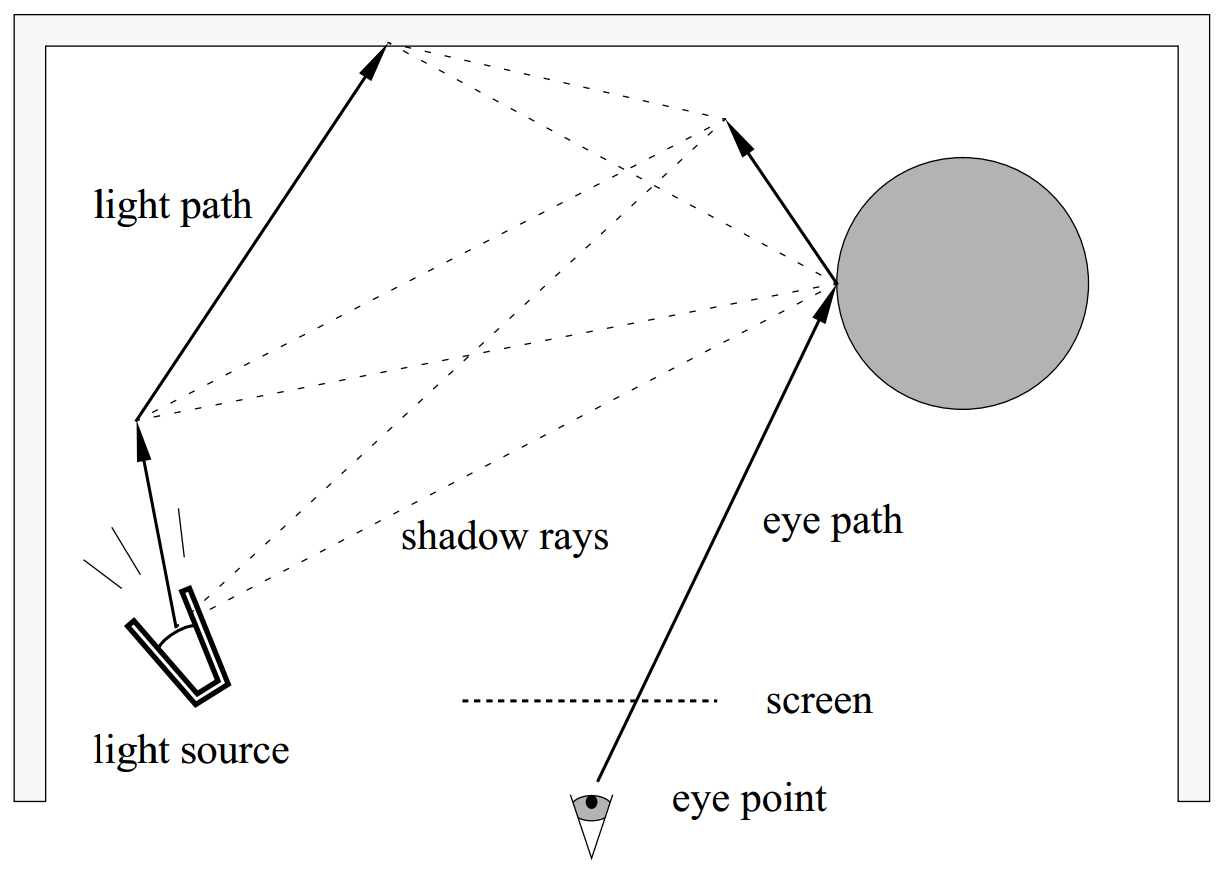
\includegraphics[width=\textwidth]{imgs/schemes/generalized_BDPT_lafortune}
        \caption{general}
        \label{fig:bdptgeneral}
    \end{subfigure}
    \begin{subfigure}{0.45\textwidth}
        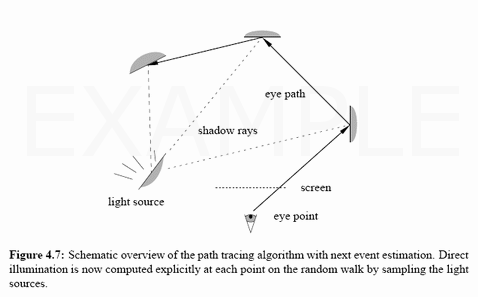
\includegraphics[width=\textwidth]{imgs/schemes/PT2_resize}
        \caption{special}
        \label{fig:udpt_ptdl}
    \end{subfigure}

    \caption{BDPT temp illustrations}
    \label{fig:bdpt}
\end{figure}


Next Event Estimation (\gls{NEE}) is one of the common methods of reducing a
variance of the path tracing. The main idea of the \gls{NEE} is to estimate
\textit{direct illumination} by sampling the light source directly at each step
of the path tracing. Then, the shadow test ray is needed to ensure that the
current light sampling position in visible by the surface.

\gls{NEE} can also be considered as the special case of the general
Bidirectional Path Tracing algorithm \gls{BDPT} \cite{Veach:94:BDPT}.
Using the vocabulary of the original paper, NEE algorithm is
\textit{(m,2)-method}. with the length of light path equals 2 and length of the
eye path $m\geq3$ is defined by the \gls{UDPT} settings.

\subsection{Volumetric Path Tracing}
\label{section:vol_path}
Path tracing with light scattering inside the media

Solving the transport equation using Monte Carlo involves a recursive
application of MC integration to evaluate the integral on the right hand side.

-To estimate the radiance at r, we sample a phase-space position r� at random,
evaluate the integrand and divide by the pdf of choosing r�. This involves
evaluating the transport kernel and also the radiance at r�. But the radiance at
r� is unknown and we have to again evaluate it using a recursive MC
estimation of the integral, this time at r�.

-This leads to the classic random walk as we know it from the path tracing
algorithm.

\subsection{Volumetric path tracing with Next Event Estimation}
The idea of direct liqght sampling can be applied to the volumetric path tracing as well.
The generalized theory of \gls{BDPT} in participating media was first described by Lafortune ans
Willems in \cite{Lafortune:1996:RPM:275458.275468}.

\ldots

Preforming the direct light estimation from inside the media with the refractive boundary proved to
be a non-trivial task.
Due to the refraction on the boundary between materials with different index of refraction
(\gls{IOR}), the light from the emitter to the scattering point never travels by a straight light.
Except the casse of the normal incident rays. To satisfy the Fermat's principle \footnote{Fermat's
principle or the principle of least time states that the path taken between two points by a ray of
light is the path that can be traversed in the least time} we have to construct the path with the
middle point somewhere on the boundary.

To my knowledge, there are no robust and fast enough methods for solving this complication in
general way. Although, there are considerable iterative approaches described in the literature
during last years \cite{holzschuch:hal-01083246}, \cite{10.1111:cgf.12681}, \cite{Koerner2016}.

In this work I have decided to consider the situation when the boundary refraction can be neglected.
In the other words, the materials with \gls{IOR}=1.
It leads to the approximation of the direct light path from inside the media to the light source as
a straight line. This assumption certainly introduces an error in the simulation. But the error is
significant only for optically low dense materials. Light propagation in highly scattering media, in
contrast, is characterized by many scattering events. Which makes the direction of the first ray
less important for the future light simulation.

\section{Intuition behind Diffusion approximation and BSSRDF formulation}
\label{section:BSSRDF_intuition}
It is clear that for most of the real world problems the analytic solution of the radiative transfer
equation is not possible. Mont Carlo integration gives correct results for the majority of the
complex scenarios but often takes too much time to compute. Especially for highly scattering media,
where the number of events can reach the order of thousands.

Diffusion approximation is particularly suitable method fo solving light simulation in highly
participating media. It gives much faster solution than classic random walks simulation, but has
some applicability limitations.

The first application of the Diffusion Approximation for computer graphics was probably mentioned in
work \cite{Stam1995}. But the main source of the practical solutions for many years was the work
\emph{A Practical Model for Subsurface Light Transport} \cite{Jensen:2001:PMS:383259.383319} Using
of the diffusion approximation is similar to using a normal distribution to estimate the result of
the sum of random variables according to Central Limit Theorem \cite{Glynn1990145}.

Two main conditions apply for reasonable usage of Diffusion Approximation to solve light scattering
in media \cite{wang2007biomedical}:
\begin{itemize}
  \item The number of scattering events is much larger than a number of absorption events. In
  addition to that, after a large number of scattering events the the radiance becomes isotropic.
  \item The mean free scattering path length is much smaller than the characteristic length of the
  change of radiance.
\end{itemize}

In the other words, only high scattering, high albedo materials (with low attenuation) for geometric
objects with with characteristic size much larger than the scattering length can be rendered with
Diffusion Approximation reasonably well.

\begin{figure}[h]
    \centering
    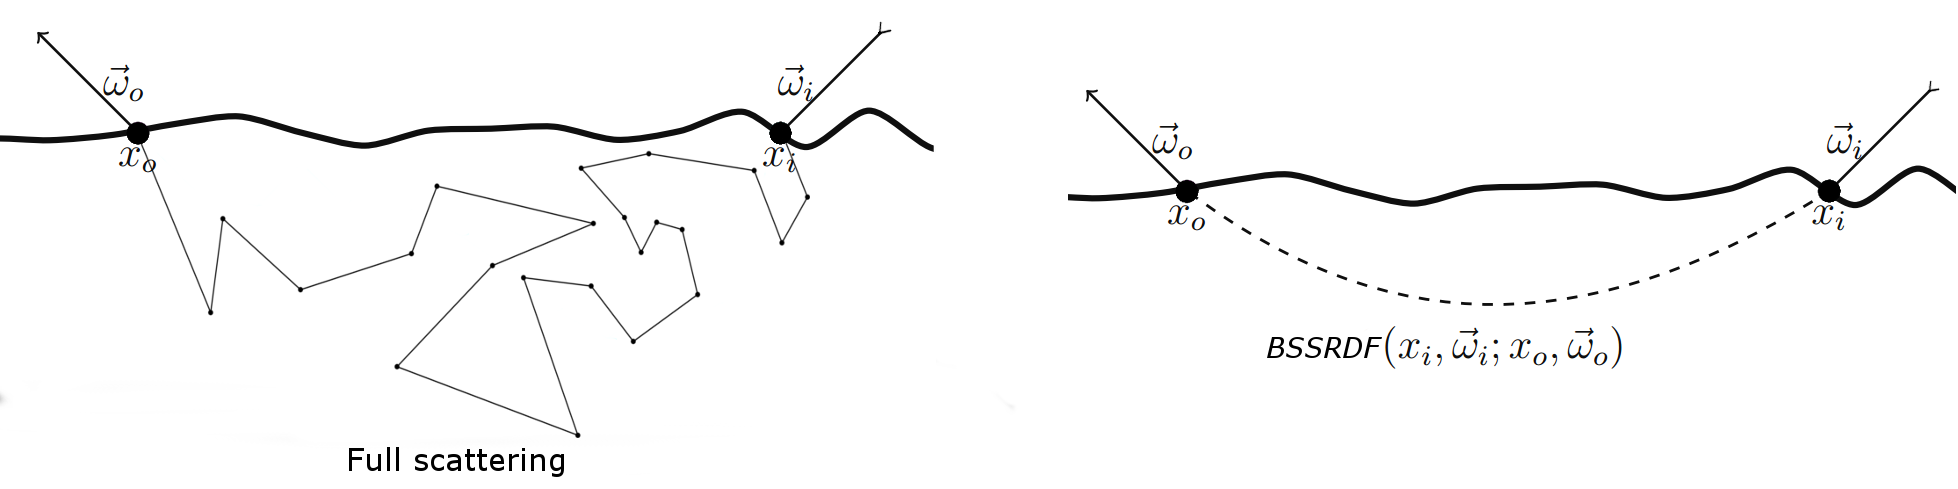
\includegraphics[width=0.9\textwidth]{schemes/bssrdf_path}
    \caption{The full scattering within the media can be approximated by the precomputed attenuation
    function}
    \label{fig:bssrdf_path}
\end{figure}

For practical usage of the Diffusion Approximation the concept of Bidirectional Subsurface
Scattering Reflectance distribution Function is often used \cite{Jensen:2001:PMS:383259.383319}.

The complex and computationally expensive process of simulating the multiple scattering in the media
can be approximated by the function which accounts for the attenuation of the radiance between
incoming and outgoing points on the surface. This approximation usually is computed with the
assumption of the flat semi-infinite surface. This is reasonable a reasonable limitation only if
scattering distance is small with respect to surface curvature and thickness. In the original work
by Jensen \cite{Jensen:2001:PMS:383259.383319} about \emph{Dipole approximation} and many other
improvements like \emph{Multipole} \cite{Donner:2005:LDM:1186822.1073308}, \emph{Quantized
diffusion} \cite{D'Eon:2011:QMR:1964921.1964951} the complex multiple scattering is approximated and
single scattering effects are still computed as a separate term.


\section{Scattering in thin objects}
Highly diffusive Bidirectional Transmission Distribution Function (BTDF) can be used as a fast
approximation of subsurface scattering in thin materials. Many real world objects like sheets of
paper or foliage of the trees has strong scattering component. There is a simple and inexpensive
technique to approximate scattering in such objects by using the Lambertian BTDF. Apart from that,
there are other more correct methods described in the literature. The recent work on the rendering
of the paper material \cite{DBLP:journals/cgf/PapasMJ14} can be seen as the further advances of the
earlier research of representation of translucent materials \cite{Donner:2005:LDM:1186822.1073308}.
